\documentclass[aspectratio=169,11pt]{beamer}
\usetheme[progressbar=frametitle,numbering=fraction,block=fill]{metropolis}
\usepackage[T1]{fontenc}
\usepackage{booktabs}
\usepackage{tabularx}
\usepackage{xcolor}
\usepackage{listings}
\usepackage[most]{tcolorbox}
\usepackage{tikz}
\usetikzlibrary{arrows.meta,positioning,calc}
\usepackage{xspace}

\graphicspath{{../../figs/}}

\definecolor{accent}{HTML}{1F5FAD}
\definecolor{good}{HTML}{2E7D32}
\definecolor{warn}{HTML}{C62828}
\definecolor{codebg}{gray}{0.95}
\setbeamercolor{alerted text}{fg=accent}
\setbeamerfont{footnote}{size=\tiny}

\lstset{basicstyle=\ttfamily\scriptsize,backgroundcolor=\color{codebg},frame=single,framerule=0pt,
        breaklines=true,columns=fullflexible,keepspaces=true,showstringspaces=false,
        keywordstyle=\color{accent}\bfseries,commentstyle=\color{gray}\itshape}

\newcommand{\pg}{PostgreSQL\xspace}
% A box to be replaced with our own screenshot / evidence before the meeting.
% \placeholder{width}{height}{what to put here}{where to get it}
\newcommand{\placeholder}[4]{%
  \begin{tcolorbox}[enhanced,width=#1,height=#2,valign=center,halign=center,
      colback=orange!4,colframe=orange!75!black,boxrule=0.8pt,arc=2pt,
      borderline={0.6pt}{0pt}{orange!75!black,dashed},frame hidden]
    \centering\footnotesize\textbf{\textcolor{orange!75!black}{PLACEHOLDER}}\\[2pt]
    #3\\[2pt]{\scriptsize\color{gray}#4}
  \end{tcolorbox}}

\title{LLM-Guided Grammar-Aware Fuzzing of PostgreSQL}
\subtitle{CS-5187 Term Project A3 --- Progress meeting 2}
\author{Venu \and Bhuvan \and Gowtham}
\date{26--30 October 2026}

\begin{document}

\maketitle

% -------------------------------------------------------------------
\begin{frame}{Status at a glance}
\begin{columns}[T]
\column{0.5\textwidth}
\textbf{Done since meeting 1}
\begin{itemize}\small
  \item Every item of the meeting-1 plan implemented and tested on real \pg master
  \item \alert{2 previously unknown \pg bugs}, root-caused, with patches
  \item 12 metamorphic oracle kinds on derivation trees, 18 plan variants, cross-version
  \item Triage: tree + token reduction, localization, upstream drafts
  \item Gated LLM arm; 23-bug re-injected benchmark
  \item Paper drafted (all five graded parts)
\end{itemize}
\column{0.5\textwidth}
\textbf{Numbers}
\begin{itemize}\small
  \item 99.5--99.7\% valid statements
  \item 20/23 benchmark bugs observable, only 9 by crashes
  \item 3{,}379 checks of new oracle kinds: 0 false positives
  \item Tree reduction: 116 $\rightarrow$ \alert{79} tokens
  \item 138 unit tests, $\approx$10.5k lines of Python
\end{itemize}
\textbf{Next}: overnight campaigns (RQ1--RQ4), file both bugs upstream
\end{columns}
\end{frame}

% -------------------------------------------------------------------
\begin{frame}{Recap: problem and the three claims}
\textbf{Problem.} \pg's planner changes every week. The worst bugs are
\alert{silent wrong results}. Crash fuzzers miss them; SQLancer-style oracles use
small hand-written generators; neither knows what changed in yesterday's commit.

\medskip
\begin{enumerate}
  \item \textbf{One tree, four jobs.} A typed derivation tree generates, mutates,
    is rewritten by the oracles, and is reduced in triage. \hfill\textcolor{good}{\textbf{all in code}}
  \item \textbf{Soundness we measure.} Generator validity; per-oracle precision
    before/after each false-positive class is fixed. \hfill\textcolor{good}{\textbf{ledger}}
  \item \textbf{The LLM proposes, the server decides.} Fragments and rewrites enter
    only through a gate on the real server. \hfill\textcolor{good}{\textbf{gate}}
\end{enumerate}

\medskip
\textbf{Ladder:} Random/Mutation $\rightarrow$ Grammar $\rightarrow$ Grammar+Oracles
$\rightarrow$ +LLM, same server, oracles, budget, seeds.
\end{frame}

% -------------------------------------------------------------------
\begin{frame}[fragile]{Motivating example: BUG-02 (found by our oracle)}
\begin{columns}[T]
\column{0.56\textwidth}
\begin{lstlisting}[language=SQL]
SELECT c,
  '(,)'::int4range @> c       AS a, -- want NULL
  'empty'::int4range @> c     AS b, -- want NULL
  NOT ('empty'::int4range @> c) AS d
FROM (VALUES (NULL::int), (1)) v(c);
-- 17, 18.6, master: NULL row ->  t | f | t
\end{lstlisting}
\small
\begin{itemize}
  \item Strict operator, but a planner \emph{support function} folds it to
    \texttt{true}/\texttt{false} (\texttt{rangetypes.c})
  \item Silent wrong result in released \pg 17 and 18
  \item Found because the oracle knew \texttt{'(,)'::int4range} is one typed
    \texttt{expr<int4range>} node: \texttt{e} $\equiv$ \texttt{(SELECT e)}
\end{itemize}
\column{0.42\textwidth}
\placeholder{\linewidth}{4.6cm}{Screenshot: \texttt{psql} on 18.6 and master
running this query, plus \texttt{EXPLAIN VERBOSE} showing \texttt{Output: true}}{docs/bughunt/BUG-02-*.md}
\end{columns}
\end{frame}

% -------------------------------------------------------------------
\begin{frame}{What changed since meeting 1}
\scriptsize\renewcommand{\arraystretch}{1.1}
\begin{tabularx}{\textwidth}{lXl}
\toprule
Plan item & What we built & Status \\
\midrule
Metamorphic oracles & TLP (WHERE, HAVING, aggregates), NoREC, expression, predicate, NOT NULL, ORDER BY, CTE, fence & \textcolor{good}{done} \\
Cross-version & master vs 18.6, per-worker DBs, intended-change list & \textcolor{good}{done} \\
Triage & reproduce $\times3$, tree + token reduction, localization, upstream draft, bisect & \textcolor{good}{done} \\
LLM loop & miner, cached prompt, gate, diff coverage, repair, ledger, rewrite gate & \textcolor{good}{done} \\
Benchmark (RQ3) & 23 reverted fixes; fixed / solo / injected servers; attribution & \textcolor{good}{done} \\
Stretch goals & plan-shape guidance, bandit weights, data profile, RLS and CERT oracles & \textcolor{good}{done} \\
Campaigns & RQ1--RQ4 configs; smoke runs pass & \textcolor{orange!80!black}{running next} \\
Upstream & BUG-01, BUG-02 patches with regression tests & \textcolor{orange!80!black}{filing this week} \\
\bottomrule
\end{tabularx}
\end{frame}

% -------------------------------------------------------------------
\section{The system}

\begin{frame}{Architecture}
\centering
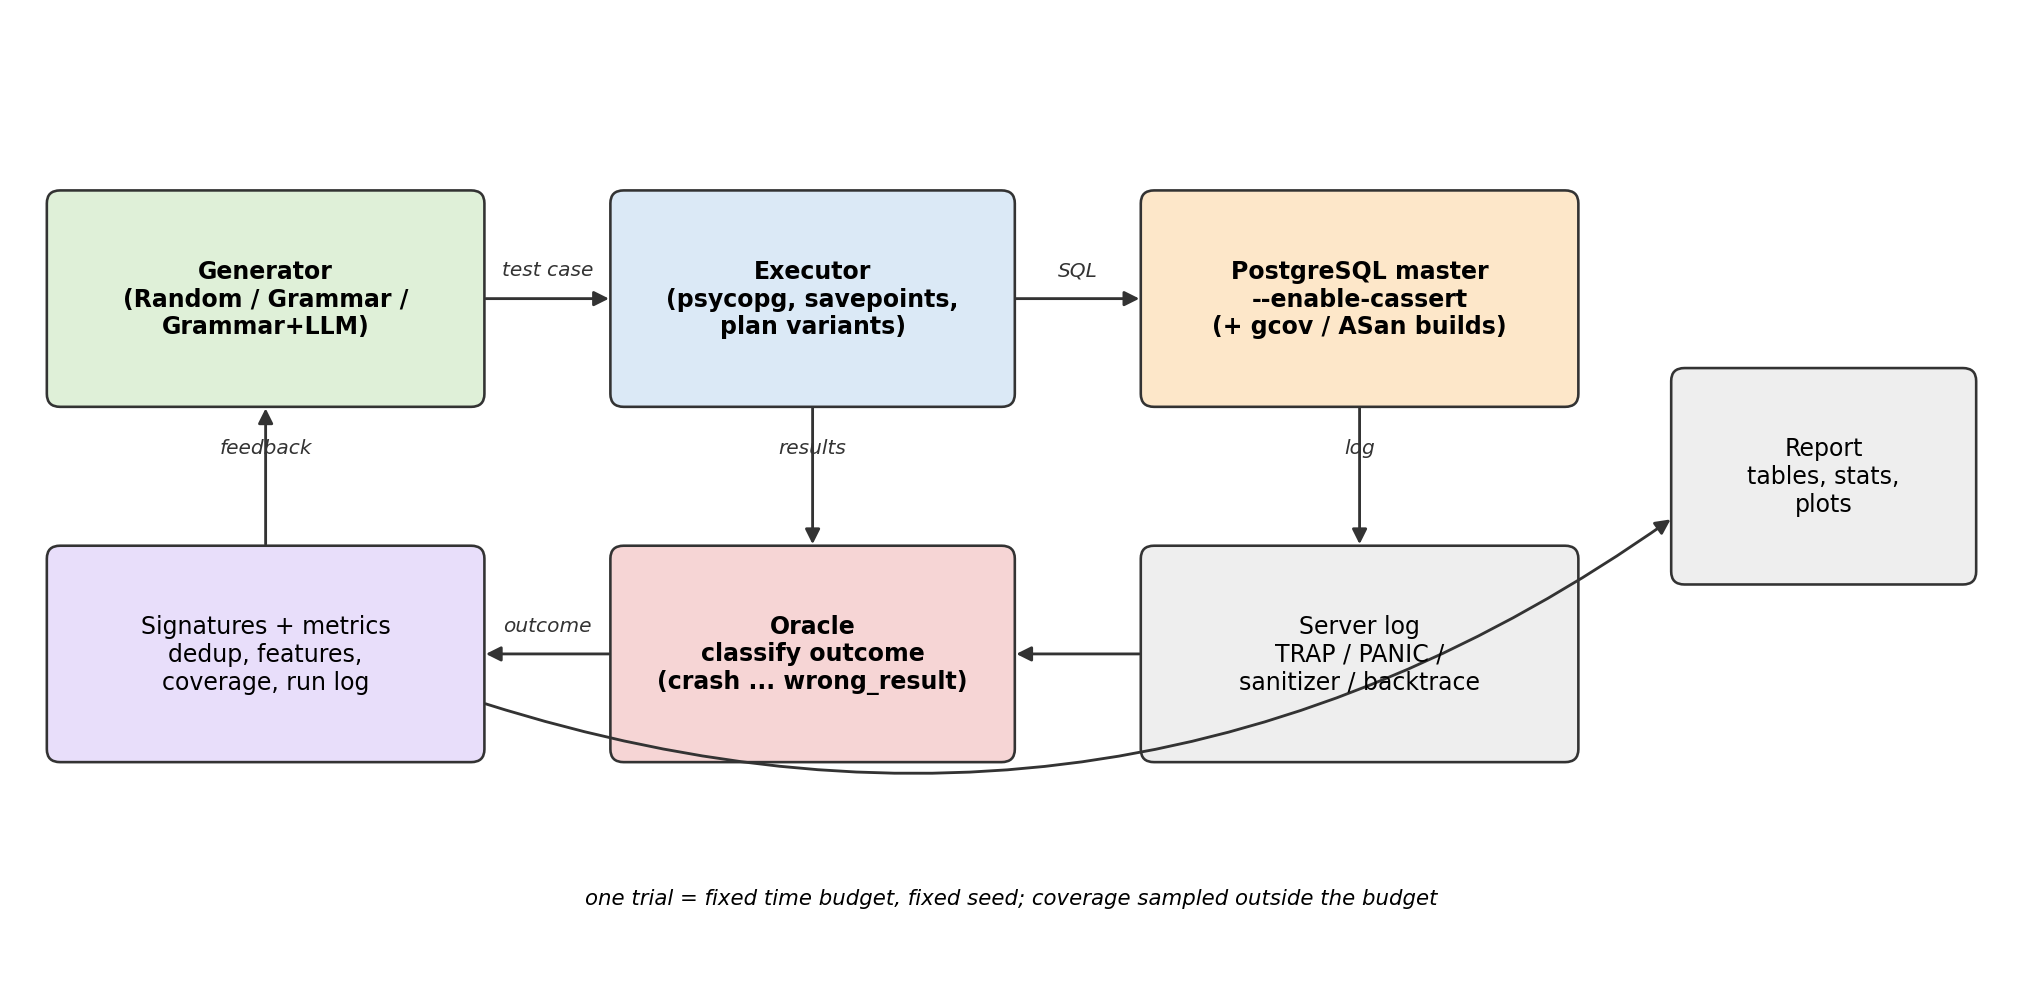
\includegraphics[width=0.92\textwidth]{architecture.png}

\small Fuzzing loop (top): derive $\rightarrow$ attach checks $\rightarrow$ run several ways
$\rightarrow$ classify/triage. LLM loop (bottom): commit $\rightarrow$ proposal $\rightarrow$ gate $\rightarrow$ grammar.
\end{frame}

\begin{frame}{One tree, four jobs}
\centering
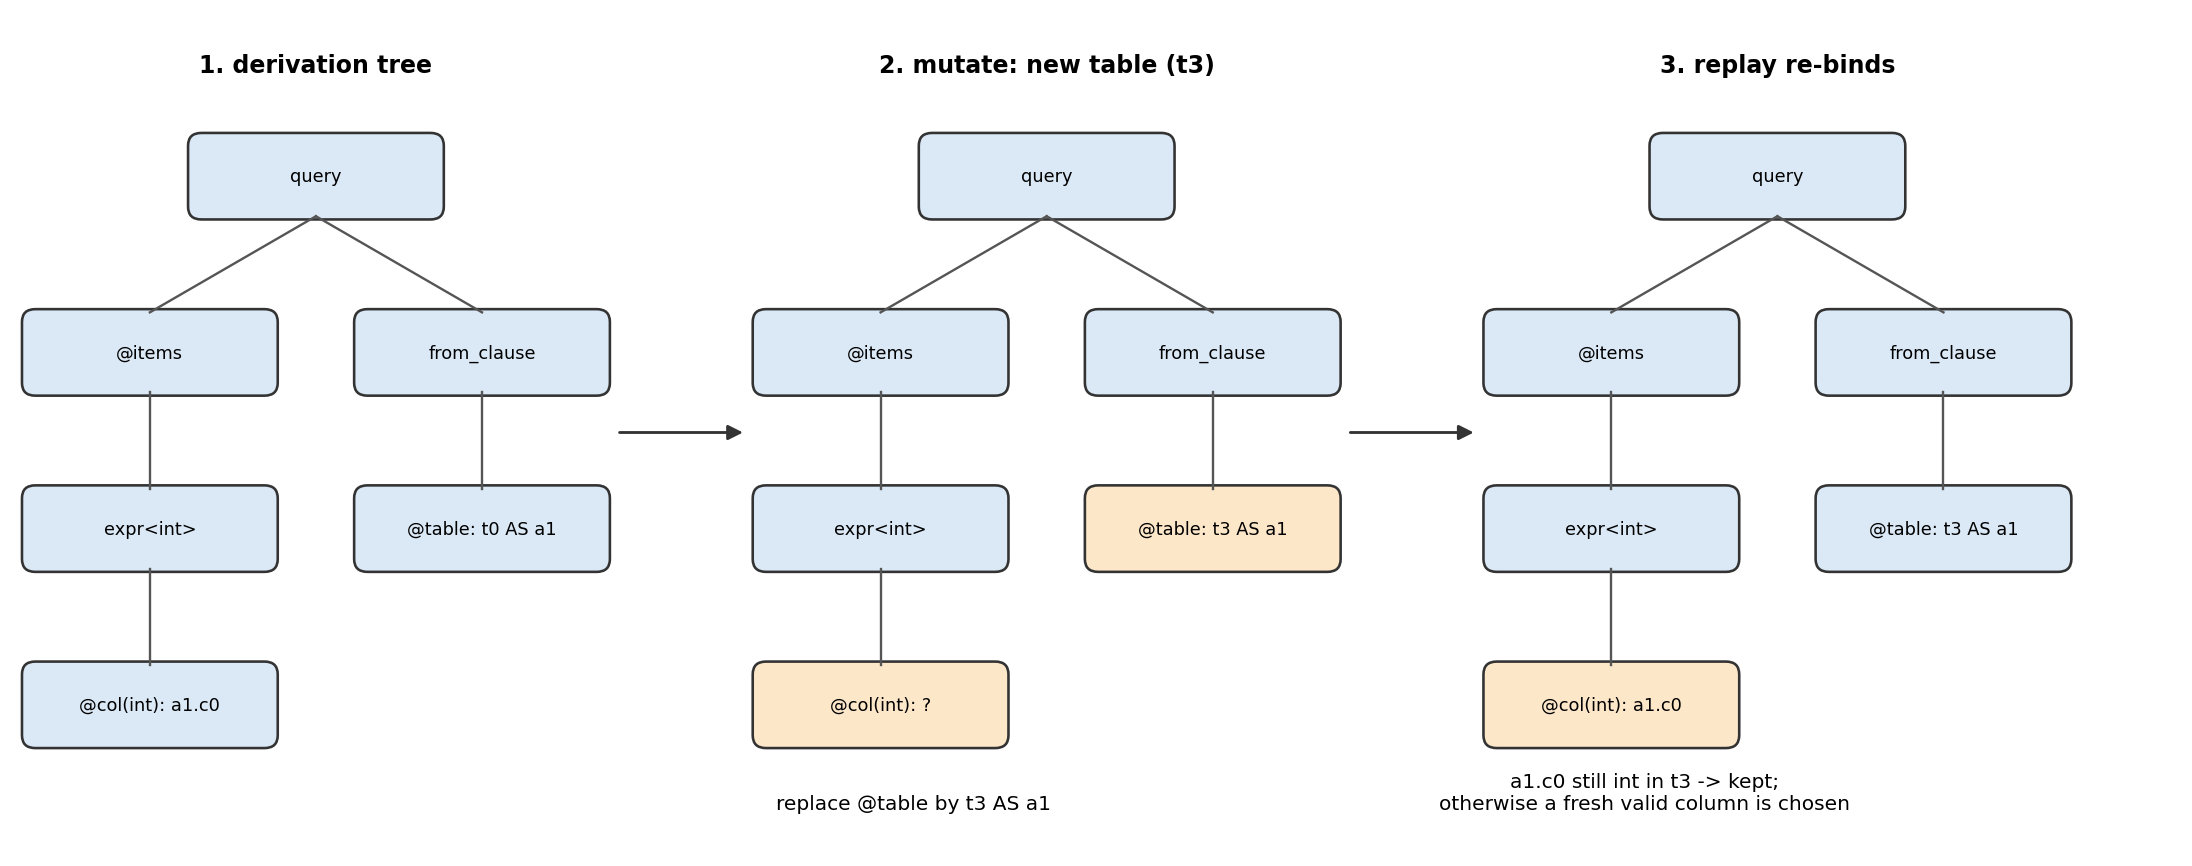
\includegraphics[width=0.8\textwidth]{grammar_replay.png}

\small
\begin{tabularx}{\textwidth}{lX}
\textbf{Generate} & typed grammar: 78 rules, 421 alternatives, scopes + type variables \\
\textbf{Mutate} & regen / splice / insert / drop subtrees; \emph{replay} re-binds names and types \\
\textbf{Oracle} & rewrite one typed node or clause span $\rightarrow$ equivalent query \\
\textbf{Reduce} & replace subtrees by their smallest derivation; replay keeps SQL valid \\
\end{tabularx}
\end{frame}

\begin{frame}{The oracle stack}
\begin{columns}[c]
\column{0.5\textwidth}
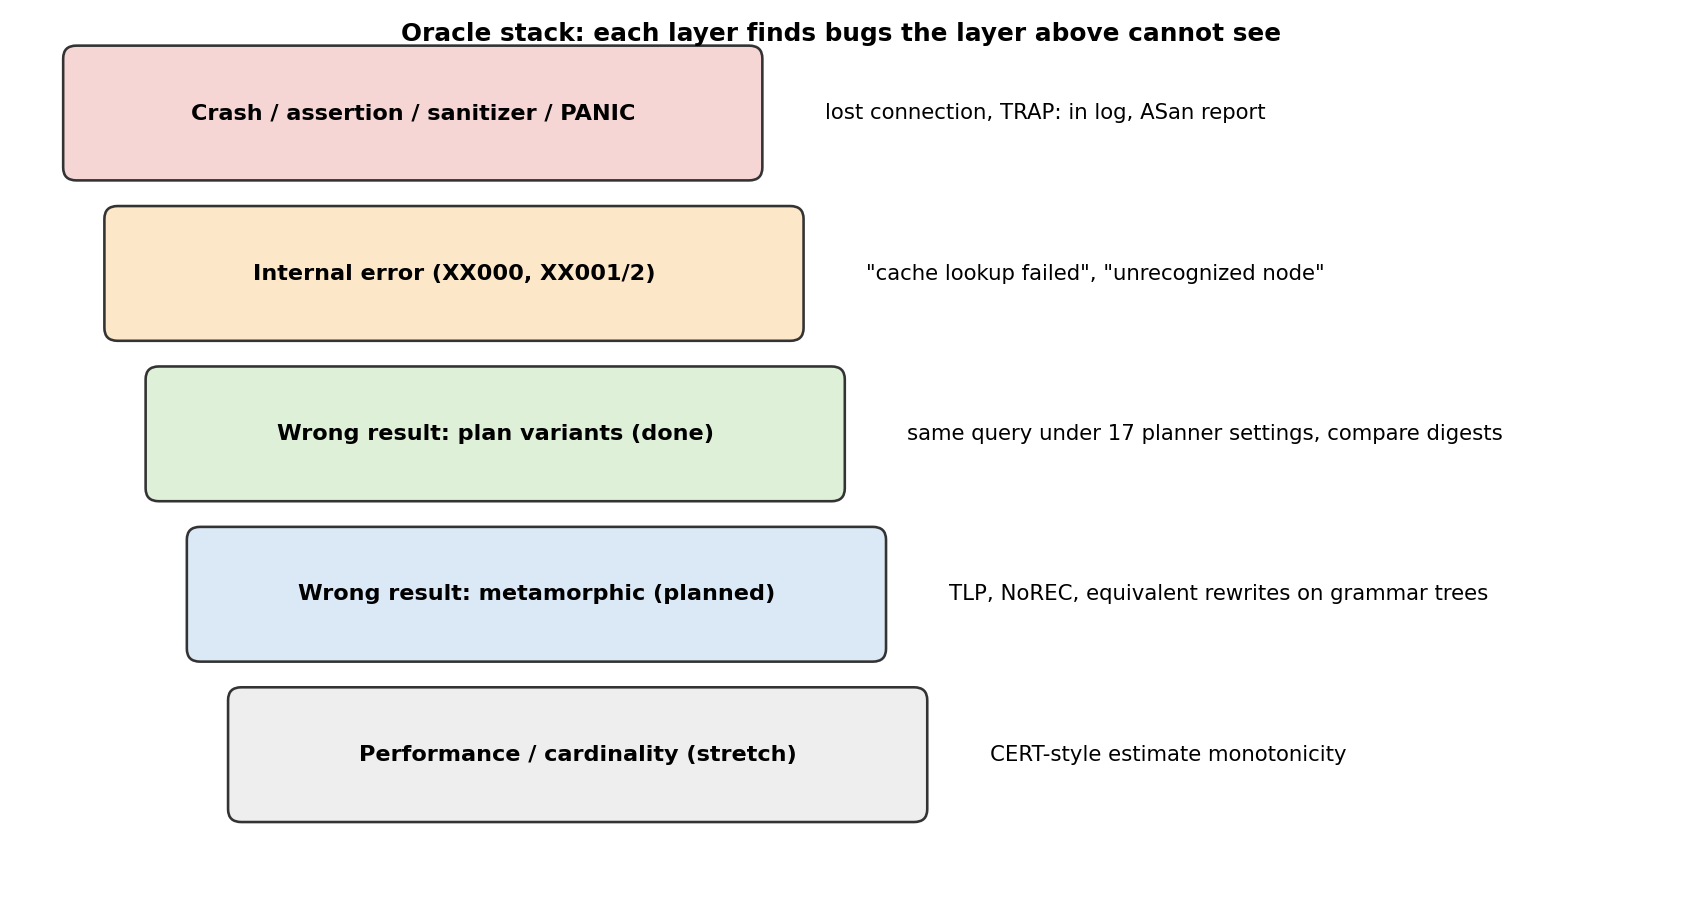
\includegraphics[width=\linewidth]{oracle_stack.png}
\column{0.5\textwidth}
\small
\begin{itemize}
  \item \textbf{Crash / assertion / internal error} on every statement (cassert build, log + PID check)
  \item \textbf{18 plan variants}: join methods, hash agg, parallel, partition-wise, tiny \texttt{work\_mem}, self-join elim., eager agg, JIT, \dots
  \item \textbf{12 metamorphic kinds} on the tree
  \item \textbf{Cross-version}: master vs 18.6
  \item Determinism filter, canonical digests (numeric scale, $-0$, float classes), confirmation re-run
\end{itemize}
\end{columns}
\end{frame}

\begin{frame}[fragile]{Metamorphic rewrites on derivation trees}
\begin{columns}[T]
\column{0.5\textwidth}
\textbf{TLP-WHERE} (generated + rewritten by the tool)
\begin{lstlisting}[language=SQL]
SELECT t0_1.c0 FROM t0 AS t0_1
  ==
(SELECT .. WHERE (t0_1.c0 > 5))
UNION ALL (SELECT .. WHERE NOT (t0_1.c0 > 5))
UNION ALL (SELECT .. WHERE (t0_1.c0 > 5) IS NULL)
\end{lstlisting}
\small
Also: TLP-HAVING, TLP-aggregates (MIN of MINs, SUM of COUNTs), NoREC,
\texttt{IN}$\leftrightarrow$\texttt{OR}, \texttt{a<b}$\leftrightarrow$\texttt{NOT(a>=b)},
\texttt{BETWEEN}, NOT NULL conjunct, drop \texttt{ORDER BY}, CTE (not) materialized,
\texttt{OFFSET 0} fence, typed expression identities.
\column{0.48\textwidth}
\begin{block}{Why the tree matters}
\small
The tree knows \emph{which} \texttt{WHERE} belongs to which \texttt{SELECT}, each
node's type, grouped levels, scopes and outer joins. So each rewrite is applied
only where it is sound:
\begin{itemize}
  \item multiset contexts only
  \item \texttt{DISTINCT}: unique-text types only
  \item NOT NULL: never under outer joins
  \item \texttt{e+0} on \texttt{int}, not on \texttt{float8}
\end{itemize}
\end{block}
\end{columns}
\end{frame}

\begin{frame}{Beyond wrong results: RLS leak oracle and CERT}
\begin{columns}[T]
\column{0.5\textwidth}
\textbf{RLS leak oracle} (information flow, L21--22)
\small
\begin{itemize}
  \item Policies on 5 tables, role \texttt{pgfuzz\_rls} (sees 131 of 203 rows of \texttt{t0})
  \item Left: query as the restricted role
  \item Right: query as superuser with each table replaced by
    \texttt{(SELECT * FROM t WHERE policy)}
  \item More rows on the left = \alert{leak}
  \item 532 checks, 0 false positives
\end{itemize}
\column{0.5\textwidth}
\textbf{CERT} (Ba \& Rigger, ICSE'24)
\small
\begin{itemize}
  \item Adding \texttt{WHERE} must not \emph{raise} the planner's row estimate
  \item Outcome \texttt{performance}, reported apart from wrong results
  \item 58 checks, 0 violations
\end{itemize}
\medskip
\normalsize\textbf{Cross-version}\\
\small 1{,}155 comparisons, 0 mismatches after fixing clock data and
excluding intended changes (\texttt{corr} on master)
\end{columns}
\end{frame}

\begin{frame}{Triage: from failure to upstream report}
\begin{center}
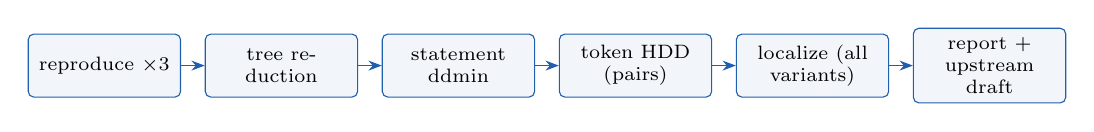
\begin{tikzpicture}[font=\scriptsize,node distance=3mm,
  b/.style={draw=accent,rounded corners=2pt,fill=accent!6,align=center,minimum height=8mm,text width=17mm}]
\node[b] (a) {reproduce $\times3$};
\node[b,right=of a] (b) {tree reduction};
\node[b,right=of b] (c) {statement ddmin};
\node[b,right=of c] (d) {token HDD (pairs)};
\node[b,right=of d] (e) {localize (all variants)};
\node[b,right=of e] (f) {report + upstream draft};
\foreach \x/\y in {a/b,b/c,c/d,d/e,e/f} \draw[-{Stealth},accent] (\x)--(\y);
\end{tikzpicture}
\end{center}
\begin{columns}[T]
\column{0.5\textwidth}
\small
\begin{tabular}{lrr}
\toprule
BUG-01 case (590 tokens) & tokens & runs \\
\midrule
token reduction only & 116 & 406 \\
tree first, then tokens & \alert{\textbf{79}} & 555 \\
\bottomrule
\end{tabular}
\begin{itemize}
  \item Localization: BUG-02 $\rightarrow$ ``not toggled by planner settings''
    $\rightarrow$ support function (correct)
\end{itemize}
\column{0.48\textwidth}
\placeholder{\linewidth}{3.6cm}{Screenshot: \texttt{pgfuzz triage} output and
the generated \texttt{upstream\_report.txt}}{results/triage/<signature>/}
\end{columns}
\end{frame}

\begin{frame}{The LLM arm: the LLM proposes, the server decides}
\begin{columns}[T]
\column{0.42\textwidth}
\footnotesize
\begin{enumerate}
  \item Mine master commits (planner, executor, parser), \alert{excluding the 23 benchmark fixes}
  \item Cached 9k-token prompt + commit digest $\rightarrow$ fragment, seeds, rewrites (JSON schema)
  \item \textbf{Gate}: parse $\cdot$ derivable ($\geq$5 uses) $\cdot$ valid on server ($\geq$60\%) $\cdot$ seeds run $\cdot$ diff coverage up
  \item Repair rounds with the server's errors (max 3); ledger of tokens and cost
\end{enumerate}
API or manual mode; stored responses replay for free.
\column{0.56\textwidth}
\textbf{Rewrite gate} (value probe + 150 live test cases)
\scriptsize\setlength{\tabcolsep}{3pt}
\begin{tabularx}{\linewidth}{@{}Xr@{}}
\toprule
Proposed rewrite & Result \\
\midrule
\texttt{CASE WHEN e IS NULL THEN NULL ELSE e END} & \textcolor{good}{accepted, 90/90} \\
\texttt{substr(e, 1)} & \textcolor{good}{accepted, 88/88} \\
\texttt{e + 1} & \textcolor{warn}{rejected: 12 mismatches} \\
\texttt{e IS TRUE} & \textcolor{warn}{rejected: probe at NULL} \\
\bottomrule
\end{tabularx}

\small\medskip
\texttt{e IS TRUE} passed 109 sampled checks: \alert{sampling is not proof}.
\end{columns}
\end{frame}

% -------------------------------------------------------------------
\section{Evaluation}

\begin{frame}{RQ3 benchmark: 23 real bugs put back into \pg}
\begin{columns}[T]
\column{0.52\textwidth}
\small
\begin{itemize}
  \item Fixes from 31 Jul--16 Oct 2026 with regression tests, reverted on base \texttt{26bd08fb}
  \item Servers: \textbf{fixed}, \textbf{solo}$_i$ (one bug), \textbf{injected} (all 23)
  \item \texttt{bench verify}: symptom = fixed vs solo difference
  \item \texttt{bench attribute}: replay finding on each solo server
\end{itemize}
\begin{block}{Key fact}
\textbf{20/23 observable, only 9 visible to a crash-only fuzzer.}
\end{block}
\column{0.46\textwidth}
\footnotesize
\begin{tabular}{lr}
\toprule
Symptom & Bugs \\
\midrule
wrong result & \alert{8} \\
internal error & 5 \\
assertion & 4 \\
missing / wrong error & 3 \\
not observable (excluded) & 3 \\
\bottomrule
\end{tabular}
\vspace{2mm}
\placeholder{\linewidth}{2.4cm}{Screenshot: \texttt{bench verify} table (fixed / solo / injected per bug)}{src/bench/reinjected/verify.json}
\end{columns}
\end{frame}

\begin{frame}{Smoke run 2: 15 min per arm on the injected server}
\small
\begin{tabular}{lrrrrr}
\toprule
Arm & Test cases & Valid & Features & Plan shapes & Bench bugs \\
\midrule
Random/Mutation & 174{,}104 & 26.3\% & 17 & 22 & 0 \\
Grammar & 16{,}841 & 99.6\% & 101 & 5{,}416 & 0 \\
Grammar+Oracles & 15{,}861 & 99.7\% & 101 & 5{,}968 & \alert{1} (158 s) \\
+LLM (no fragments yet) & 15{,}800 & 99.7\% & 101 & 5{,}937 & \alert{1} (160 s) \\
\bottomrule
\end{tabular}

\medskip
\begin{itemize}
  \item 10$\times$ more test cases do not buy reach: random reaches 17 features
  \item \texttt{rb-dfcf6fa7} found only with oracles + plan guidance; attribution by replay
    separated it from a bug with the same message
  \item One trial each: this shows the pipeline works, \emph{not} a significant difference
\end{itemize}
\end{frame}

\begin{frame}{Component checks on master (single runs)}
\footnotesize
\begin{tabularx}{\textwidth}{lX}
\toprule
Component & Measured \\
\midrule
Metamorphic oracles (first run) & 907 checks, 0 FP; \alert{BUG-02 in the first 150 test cases} \\
New rewrite kinds & 798 checks, 0 false positives \\
Full system, 3 min & 3{,}166 test cases, 99.5\% valid, 1{,}991 checks, 7{,}956 variant runs, 0 FP \\
Bandit weights & 533 vs 419 plan shapes per 1{,}000 test cases, same validity \\
Data profile (\texttt{@dlit}) & selective predicates (5--95\% of rows): 29.3\% $\rightarrow$ 58.6\% \\
Tree replay & 599/600 stored trees replay to identical SQL \\
Token reduction (BUG-02) & 4 statements / 107 tokens $\rightarrow$ 1 / 36 in 307 runs \\
LLM fragment gate & valid fragment 251/251 accepted; invalid rejected with server message \\
\bottomrule
\end{tabularx}
\end{frame}

\begin{frame}{Precision ledger (RQ2, claim 2)}
\begin{columns}[T]
\column{0.55\textwidth}
\footnotesize
\begin{tabular}{lrrrr}
\toprule
Oracle & Cand. & Real & FP & After fixes \\
\midrule
assertion & 2 & 1 & 1 & 1.00 \\
crash & 1 & 0 & 1 & -- \\
cross-version & 3 & 0 & 2 & -- \\
internal error & 2 & 1 & 0 & 1.00 \\
mm: expr & 1 & 1 & 0 & 1.00 \\
mm: tlp\_having & 4 & 0 & 4 & -- \\
plan-variant & 5 & 0 & 5 & -- \\
\midrule
all & 18 & 3 & 13 & 1.00 \\
\bottomrule
\end{tabular}

\scriptsize 2 flaky. Raw precision 0.19, logged on purpose.
\column{0.43\textwidth}
\small
\textbf{6 false-positive classes, all fixed + tested}
\begin{itemize}\scriptsize
  \item \texttt{ARRAY(SELECT)} without \texttt{ORDER BY}
  \item TLP-HAVING without \texttt{GROUP BY}
  \item numeric scale under \texttt{DISTINCT}
  \item clock in seed data across versions
  \item our PoC replay crashed a shared server $\rightarrow$ PID check
  \item intended \texttt{corr} change on master
\end{itemize}
\alert{Lesson: oracle precision, not generator power, is the bottleneck.}
\end{columns}
\end{frame}

\begin{frame}{Bugs found}
\begin{columns}[T]
\column{0.5\textwidth}
\textbf{BUG-01 --- JSON\_TABLE collations}
\scriptsize
\begin{itemize}
  \item Found by the grammar campaign (assertion, \texttt{execExpr.c:2078})
  \item 18.6: \texttt{ROW(1,2) < ROW(3,4)} in the context item returns \alert{false}
  \item Missing \texttt{assign\_expr\_collations()} in \texttt{parse\_jsontable.c}
  \item One-line patch + regression tests; 17, 18, master
\end{itemize}
\column{0.5\textwidth}
\textbf{BUG-02 --- range containment w/ NULL}
\scriptsize
\begin{itemize}
  \item Found by \texttt{expr:scalar\_sub} rewrite
  \item \texttt{find\_simplified\_clause()} folds to a constant
  \item Patch: simplify only if the element is provably non-null
  \item \texttt{make check} passes; 17, 18, master
\end{itemize}
\end{columns}
\vspace{-1mm}\placeholder{\textwidth}{1.9cm}{Upstream status: pgsql-bugs numbers + thread links for BUG-01 and BUG-02}{postgresql.org/list/pgsql-bugs}
\end{frame}

\begin{frame}{Experiment design (RQ1--RQ4)}
\begin{columns}[T]
\column{0.5\textwidth}
\small
\begin{description}
  \item[RQ1] reach: validity, line/branch coverage, features, plan shapes
  \item[RQ2] bugs found and per-oracle precision
  \item[RQ3] re-injected bugs found, time to find
  \item[RQ4] what the LLM adds (diff coverage, ablation) and costs
\end{description}
\column{0.5\textwidth}
\small
\begin{itemize}
  \item RQ1: 7 arms (incl.\ no-bandit and LLM ablations) $\times$ 5 trials $\times$ 1 h, gcov build
  \item RQ3: 4 arms $\times$ 5 $\times$ 1 h, injected server + 18.6 reference
  \item Paired seeds, same oracles and budget; one commit (\texttt{26bd08fb}) for everything
  \item Medians, IQR, bootstrap 95\% CI, Mann--Whitney U, Vargha--Delaney $\hat A_{12}$
\end{itemize}
\end{columns}
\end{frame}

\begin{frame}{RQ1 results (to fill after the campaign)}
\begin{columns}[T]
\column{0.5\textwidth}
\placeholder{\linewidth}{5.2cm}{Plot: backend line coverage over time, median and IQR band per arm}{pgfuzz report ../results/rq1 $\rightarrow$ plots/}
\column{0.5\textwidth}
\placeholder{\linewidth}{5.2cm}{Table: validity, coverage, features, plan shapes per arm with $p$ and $\hat A_{12}$}{results/rq1/report.md}
\end{columns}
\end{frame}

\begin{frame}{RQ3 and RQ4 results (to fill after the campaigns)}
\begin{columns}[T]
\column{0.5\textwidth}
\placeholder{\linewidth}{5.2cm}{Table: bugs found per arm (out of 20), time to first detection per bug}{pgfuzz bench attribute $\rightarrow$ table\_rq3.tex}
\column{0.5\textwidth}
\placeholder{\linewidth}{5.2cm}{LLM ledger: fragments accepted/rejected, repair rounds, diff coverage with/without, tokens and \$}{pgfuzz llm report}
\end{columns}
\end{frame}

% -------------------------------------------------------------------
\section{Plan}

\begin{frame}{Timeline to the deadline}
\begin{center}
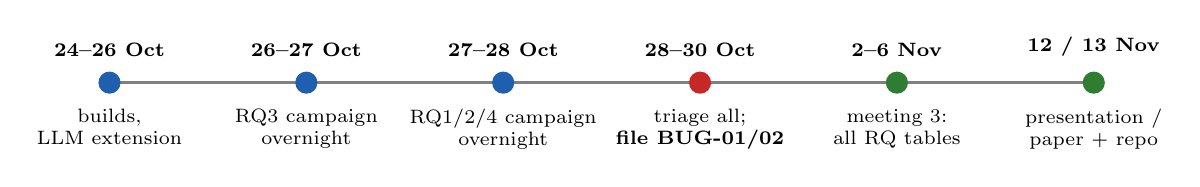
\begin{tikzpicture}[font=\scriptsize]
\draw[very thick,gray] (0,0) -- (12.5,0);
\foreach \x/\top/\bot/\c in {
  0/{24--26 Oct}/{builds,\\LLM extension}/accent,
  2.5/{26--27 Oct}/{RQ3 campaign\\overnight}/accent,
  5.0/{27--28 Oct}/{RQ1/2/4 campaign\\overnight}/accent,
  7.5/{28--30 Oct}/{triage all;\\\textbf{file BUG-01/02}}/warn,
  10.0/{2--6 Nov}/{meeting 3:\\all RQ tables}/good,
  12.5/{12 / 13 Nov}/{presentation /\\paper + repo}/good}
{
  \fill[\c] (\x,0) circle (4pt);
  \node[above=6pt,align=center] at (\x,0) {\textbf{\top}};
  \node[below=6pt,align=center] at (\x,0) {\bot};
}
\end{tikzpicture}
\end{center}
\small
\begin{itemize}
  \item Exact commands and expected times in \texttt{docs/EXECUTION\_PLAN.md}
    (phases 0--5, $\approx$16 h of machine time, $\approx$1.5 h of ours)
  \item Campaigns resume if interrupted
\end{itemize}
\end{frame}

\begin{frame}{Risks and what we would like feedback on}
\begin{columns}[T]
\column{0.5\textwidth}
\textbf{Risks and fallbacks}
\small
\begin{itemize}
  \item New false-positive classes in long runs $\rightarrow$ triage; they are RQ2 data
  \item LLM API unavailable $\rightarrow$ manual mode, replayed responses
  \item No upstream reply by 13 Nov $\rightarrow$ report filing, reproducer, patch
  \item 5 trials may not reach $p<0.05$ $\rightarrow$ effect sizes + CIs; more trials if time
\end{itemize}
\column{0.5\textwidth}
\textbf{Questions for you}
\small
\begin{itemize}
  \item Is 5 trials $\times$ 1 h per arm acceptable, or should we cut arms for 10 trials?
  \item Does a filed bug with a patch, under review by 13 Nov, count towards the top band?
  \item Paper is $\approx$1 page over 12: cut related work or component checks?
\end{itemize}
\end{columns}
\end{frame}

\begin{frame}{Live demo (backup screenshots)}
\begin{columns}[T]
\column{0.31\textwidth}
\placeholder{\linewidth}{4.2cm}{\texttt{pgfuzz sample --execute}: generated SQL and 99.5\% validity}{terminal}
\column{0.31\textwidth}
\placeholder{\linewidth}{4.2cm}{\texttt{pgfuzz triage}: 590 $\rightarrow$ 79 tokens, report}{docs/evidence/}
\column{0.31\textwidth}
\placeholder{\linewidth}{4.2cm}{RQ3 smoke report: medians, $\hat A_{12}$, time to first bug}{rq3\_smoke2/report.md}
\end{columns}
\end{frame}

\begin{frame}[standout]
Thank you --- questions?

\medskip
\normalsize github.com/v28k/cs5187-term-project
\end{frame}

\end{document}
